\documentclass[a4paper,twoside,bibtotoc,abstracton,12pt,BCOR=15mm]{article}
\usepackage[english]{babel}
\usepackage[utf8]{inputenc}
\usepackage{graphicx}
\usepackage{booktabs}
\usepackage[table]{xcolor}
\usepackage{colortbl}
\usepackage{color}
\usepackage{graphicx}
\usepackage{makeidx}  % allows for indexgeneration
\usepackage{amsmath, amssymb} % amsthm stuff also defined by llncs
\usepackage{graphicx}
\usepackage{subfig} 
\usepackage{url}
\usepackage{color}
\usepackage{booktabs}
\usepackage{listings}
\usepackage{xspace}
\usepackage{lscape}
\usepackage{listings}
\usepackage{color}
\usepackage{tabularx}
\usepackage{tikz}
\usetikzlibrary{calc,positioning,shapes.geometric,arrows,shapes}

\graphicspath{{.}{../Common/}{../../Common/}}

\def\deliverableNumber{8.4.1}
\def\deliverableTitle{Online Collaboration Platform}

\def\disseminationLevel{Public}
\def\dueDate{Month 6, 28/2/2011}
\def\submissionDate{02/3/2011}
\def\workPackage{WP8,Project Management}
\def\task{Task T8.4}
\def\type{Report}
\def\approvalStatus{Approved}
\def\version{1.0}
\def\numberOfPages{67}
\def\filename{D8.4.1\_Online\_Collaboration\_Platform\_Public.pdf}

\definecolor{lod_blue}{RGB}{192,227,242}
\definecolor{LodBlue}{rgb}{0.7529,0.8902,0.9490}

\newcommand{\orchid}{\textsc{Orchid}\xspace}
\newcommand{\geolift}{\textsc{DEER}\xspace}
\newcommand{\limes}{\textsc{Limes}\xspace}
\DeclareMathOperator*{\argmax}{arg\,max}
\DeclareMathOperator*{\argmin}{arg\,min}

%%%%%%%%%%%%%%%%%%%%%%%%%%%%%%%%%%%%%%%%%%%%%%%%%%%%%%%%%%%%%%%%%%%%%%%%%%%%%%%%%%
\definecolor{dkgreen}{rgb}{0,0.6,0}
\definecolor{gray}{rgb}{0.5,0.5,0.5}
\definecolor{mauve}{rgb}{0.58,0,0.82}

\lstset{frame=tb,
  language=Java,
  aboveskip=3mm,
  belowskip=3mm,
  showstringspaces=false,
  columns=flexible,
  basicstyle={\small\ttfamily},
  numbers=none,
  numberstyle=\tiny\color{gray},
  keywordstyle=\color{blue},
  commentstyle=\color{dkgreen},
  stringstyle=\color{mauve},
  breaklines=true,
  breakatwhitespace=true
  tabsize=3
}
%%%%%%%%%%%%%%%%%%%%%%%%%%%%%%%%%%%%%%%%%%%%%%%%%%%%%%%%%%%%%%%%%%%%%%%%%%%%%%%%%%
\begin{document}



%\small{ Making the Web an Exploratory for Geospatial Knowledge}


\vspace*{\fill} 
\begin{quote} 
\centering 
\begin{center}
 
\includegraphics[scale=0.5]{images/geoknow.png}
\end{center}
\begin{flushleft}
 \Large{\geolift}
 \small{ - RDF Data Extraction and Enrichment Framework.}
\end{flushleft}
\end{quote}
\vspace*{\fill}
\newpage

\vspace*{\fill} 
\begin{quote} 

\textbf{Abstract}: \\
Over the last years, the Linked Data principles have been used across academia and industry to publish and consume structured data. Thanks to the fourth Linked Data principle, many of the RDF datasets used within these applications contain implicit and explicit references to more data. For example, music datasets such as Jamendo include references to locations of record labels, places where artists were born or have been, etc. Datasets such as Drugbank contain references to drugs from DBpedia, were verbal description of the drugs and their usage is explicitly available. The goal of mapping component, dubbed DEER, is to retrieve this information, make it explicit and integrate it into data sources according to the specifications of the user. To this end, DEER relies on a simple yet powerful pipeline system that consists of two main components: modules and operators.

Modules implement functionality for processing the content of a dataset (e.g., applying named entity recognition to a particular property). Thus, they take a dataset as input and return a dataset as output. Operators work at a higher level of granularity and combine datasets. Thus, they take sets of datasets as input and return sets of datasets.
\geolift was implemented in Java, is open-source and can be accessed at \url{https://github.com/GeoKnow/DEER/}. 
\end{quote}
\vspace*{\fill}

\newpage
\tableofcontents
\newpage

\section{Introduction}
Manifold RDF data contain implicit references to geographic data.
For example, music datasets such as \emph{Jamendo} include references to locations of record labels, places where artists were born or have been, etc.
The aim of the spatial mapping component, dubbed \geolift, is to retrieve this information and make it explicit.
In the following, we begin by presenting the basic assumptions that influence the development of the first component of \geolift.
Then, we present the technical approach behind \geolift.
Finally, we present the detailed developers' manual of \geolift.
%in which we introduce how to deal with different modules of \geolift and integrate it with other tool.

\section{Assumptions}
Geographical information can be mentioned in three different ways within Linked Data:
\begin{enumerate}
\item \emph{Through dereferencing}: Several datasets contain links to datasets with explicit geographical information such as \emph{DBpedia} or \emph{LinkedGeoData}. 
For example, in a music dataset, one might find information such as\\ 
\texttt{http://example.org/Leipzig \\
owl:sameAs \\ 
http://dbpedia.org/resource/Leipzig}.

We call this type of reference \emph{explicit}. 
We can now use the semantics of RDF to fetch geographical information from DBpedia and attach it to the resource in the other ontology as \texttt{http://example.org/Leipzig} and \texttt{http://dbpedia.org/resource/Leipzig} refer to the same real-world object.

\item \emph{Through linking}: It is known that the Web of Data contains an insufficient number of links. 
The latest approximations suggest that the Linked Open Data Cloud alone consists of 31+ billion triples but only contains approximately 0.5 billion links (i.e., less than 2\% of the triples are links between knowledge bases). 
The second intuition behind our approach is thus to use link discovery to map resources in an input knowledge base to resources in a knowledge that contains explicit geographical information. 
For example, given a resource \texttt{http://example.org/Athen}, \geolift should aim to find a resource such as \texttt{http://dbpedia.org/resource/Athen} to map it with. 
Once having established the link between the two resources, \geolift can then resolve to the approach defined above.

\item \emph{Through Natural Language Processing}: In some cases, the geographic information is hidden in the objects of data type properties. 
For example, some datasets contain biographies, textual abstracts describing resources, comments from users, etc.
The idea here is to use this information by extracting Named Entities and keywords using automated Information Extraction techniques.
Semantic Web Frameworks such as FOX\footnote{\url{http://fox.aksw.org}} have the main advantage of providing URIs for the keywords and entities that they detect.
These URIs can finally be linked with the resources to which the datatype properties were attached.
Finally, the geographical information can be dereferenced and attached to the resources whose datatype properties were analyzed.
\end{enumerate}

The idea behind \geolift is to provide a generic architecture that contains means to exploit these three characteristics of Linked Data. 
In the following, we present the technical approach underlying \geolift.

\section{Technical Approach}
\subsection{Architecture}
\geolift was designed to be a modular tool which can be easily extended and re-purposed.
In its first version, it provides two main types of artifacts:
\begin{enumerate}
\item \emph{Modules}: These artifacts are in charge of generating geographical data based on RDF data. 
To this aim, they implement the three intuitions presented above.
The input for such a module is an RDF dataset (in Java, a \emph{Jena Model}).
The output is also an RDF dataset enriched with geographical information (in Java, an enriched \emph{Jena Model}).
Formally, a module can thus be regarded as a function $\mu: \mathcal{R} \rightarrow \mathcal{R}$, where $\mathcal{R}$ is the set of all RDF datasets.
\item \emph{Operators}: The idea behind operators is to enable users to define a workflow for processing their input dataset. 
Thus, in case a user knows the type of enrichment that is to be carried out (using linking and then links for example), he can define the sequence of modules that must be used to process his dataset.
Note that the format of the input and output of modules is identical. 
Thus, the user is empowered to create workflows of arbitrary complexity by simply connecting modules.
Formally, an operator can be regarded as a function $\varphi: \mathcal{R} \cup \mathcal{R}^2 \rightarrow \mathcal{R} \cup \mathcal{R}^2$.
\end{enumerate}
The corresponding architecture is shown in Figure~\ref{fig:architecture}. The input layer allows reading RDF in different serializations.
The enrichment modules are in the second layer and allow adding geographical information to RDF datasets by different means.
The operators (which will be implemented in the future version of \geolift) will combine the enrichment modules and allow defining a workflow for processing information.
The output layer serializes the results in different format.
The enrichment procedure will be monitored by implementing a controller, which will be added in the future version of \geolift.


\begin{figure}[ht!]
			\centering
			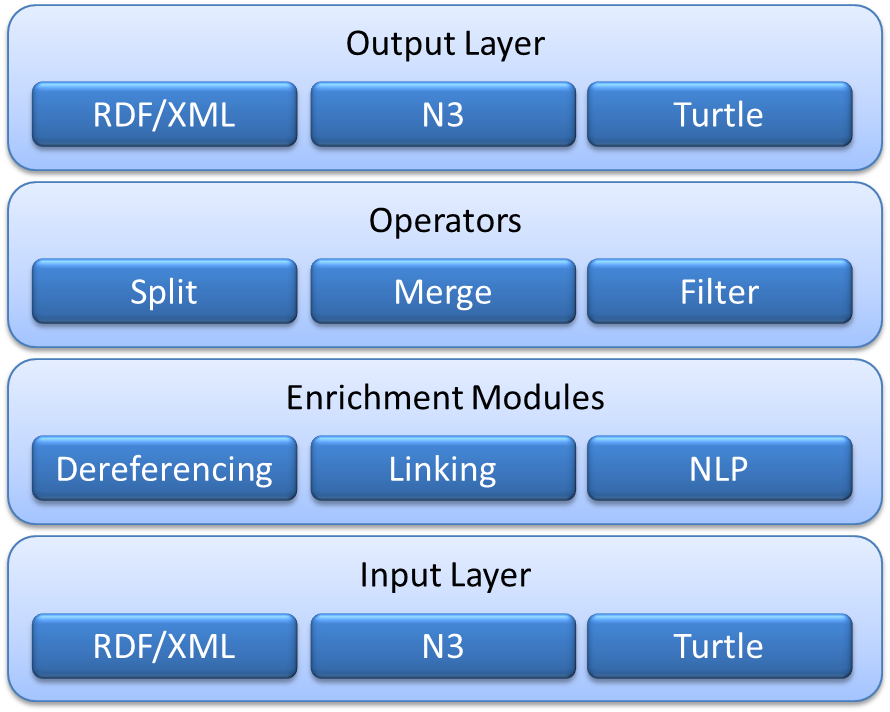
\includegraphics[width = 0.6\textwidth]{images/geolift_architecture.png}
			\caption{Architecture of \geolift}
			\label{fig:architecture}
		\end{figure}

In the following, we present the implementation of the three intuitions presented above in \geolift.
\subsection{Using Dereferencing}
For datasets which contain \texttt{owl:sameAs} links, we dereference all links from the dataset to other datasets by using a content negotiation on HTTP as shown in Figure~\ref{fig:contentNegotiation}.
This returns a set of triples that needs to be filtered for relevant geographical information.
Here, we use a predefined list of attributes that links to geographical information.
Amongst others, we look for \texttt{geo:lat}, \texttt{geo:long}, \texttt{geo:lat\_long}, \texttt{geo:line} and \texttt{geo:polygon}.
The list of retrieved property values can be configured.

\begin{figure}[htb]
\centering
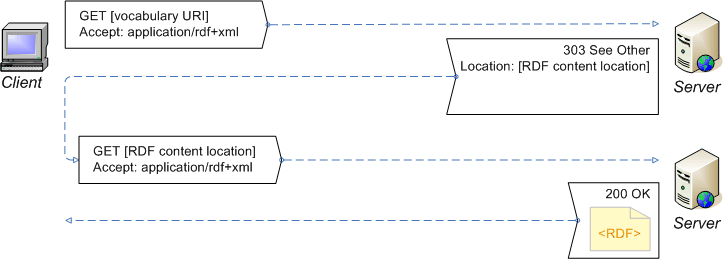
\includegraphics[width=0.7\textwidth]{images/contentnegotiation}
\caption{Content Negotiation as used by \geolift (courtesy of W3C)}
\label{fig:contentNegotiation}
\end{figure}

\subsection{Using Linking}
As pointed out before, links to geographical resources do not occur in several knowledge bases.
Here, we rely on the metrics implemented in the \limes framework\footnote{\url{http://\limes.sf.net}}~\cite{NGAU11,NGON12c,NGO+13c} to link the resources in the input dataset with geographical datasets.
\limes, the \textbf{Li}nk Discovery Framework for \textbf{Me}tric \textbf{S}paces, is a framework for discovering links between entities contained in Linked Data sources. \limes is a hybrid framework~\cite{NGON12c} that combines the mathematical characteristics of metric spaces as well prefix-, suffix- and position filtering to compute pessimistic approximations of the similarity of instances. These approximations are then used to filter out a large amount of those instance pairs that do not suffice the mapping conditions. By these means, \limes can reduce the number of comparisons needed during the mapping process by several orders of magnitude and complexity without loosing a single link.
The architecture of \limes is shown in Figure~\ref{fig:limesArchitecture}

\begin{figure}[ht!]
  \centering
  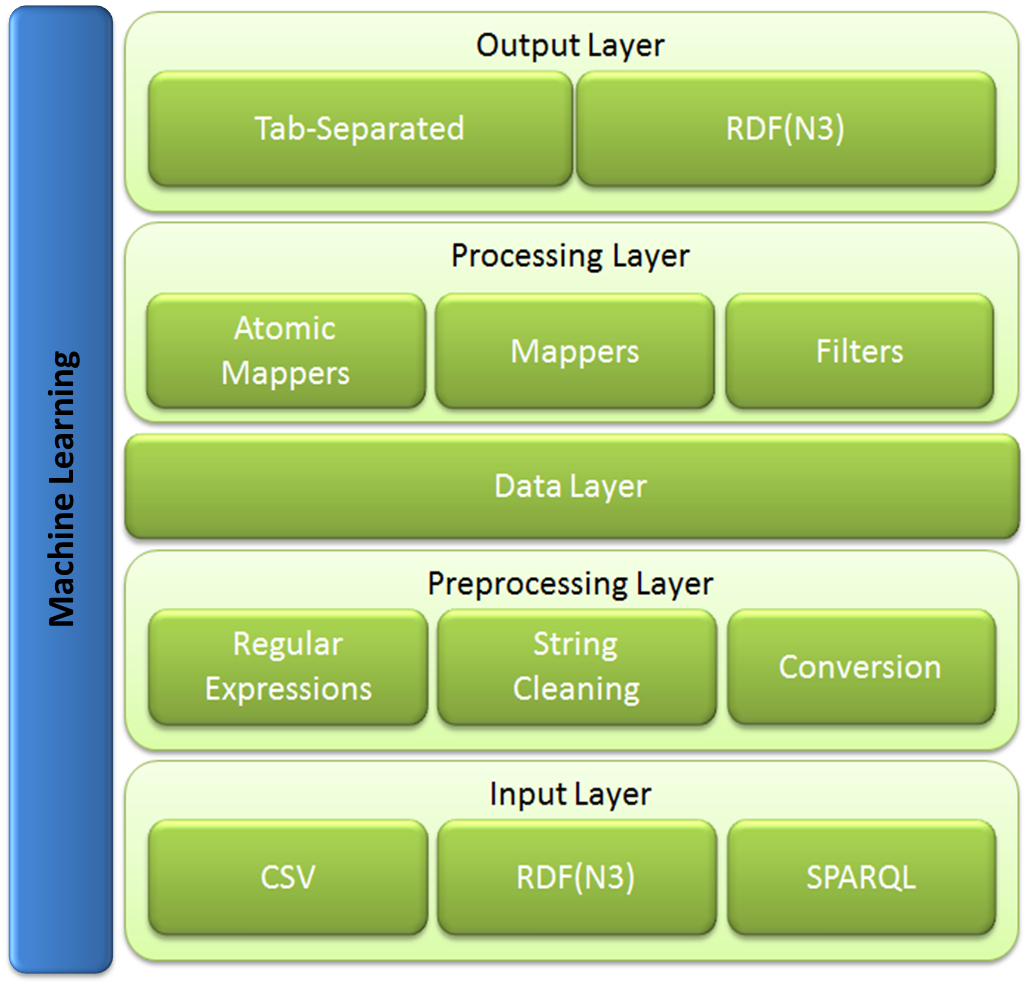
\includegraphics[width = 0.6\textwidth]{images/limesArchitecture.png}
  \caption{Architecture of \limes}
  \label{fig:limesArchitecture}
\end{figure}
		


Linking using \limes~\cite{NGON12c,NGON12} can be achieved in three ways:
\begin{enumerate}
\item \emph{Manually}, by the means of a link specification~\cite{NGON12c}, which is an XML-description of (1) the resource in the input and target datasets that are to be linked and (2) of the similarity measure that is to employed to link these datasets.
\item \emph{Semi-automatically} based on active learning~\cite{NGO+11a,NGLY12,NGO+13b}. Here, the idea is that if the user is not an expert and thus unable to create a link specification, he can simply provide the framework with positive and negative examples iteratively. 
Based on these examples, \limes can compute links for mapping resources with high accuracy.
\item \emph{Automatically} based on unsupervised machine learning. Here, the user can simply specify the sets of resources that are to be linked with each other. 
\limes implements both a deterministic and non-deterministic machine-learning approaches that optimize a pseudo-F-measure to create a one-to-one mapping.
\end{enumerate}

The techniques implemented by \limes can be accessed via the SAIM user interface\footnote{\url{http://saim.aksw.org}}, of which a screenshot is shown in Figure~\ref{fig:saim_screenshot}.
\begin{figure}[htb]
\centering
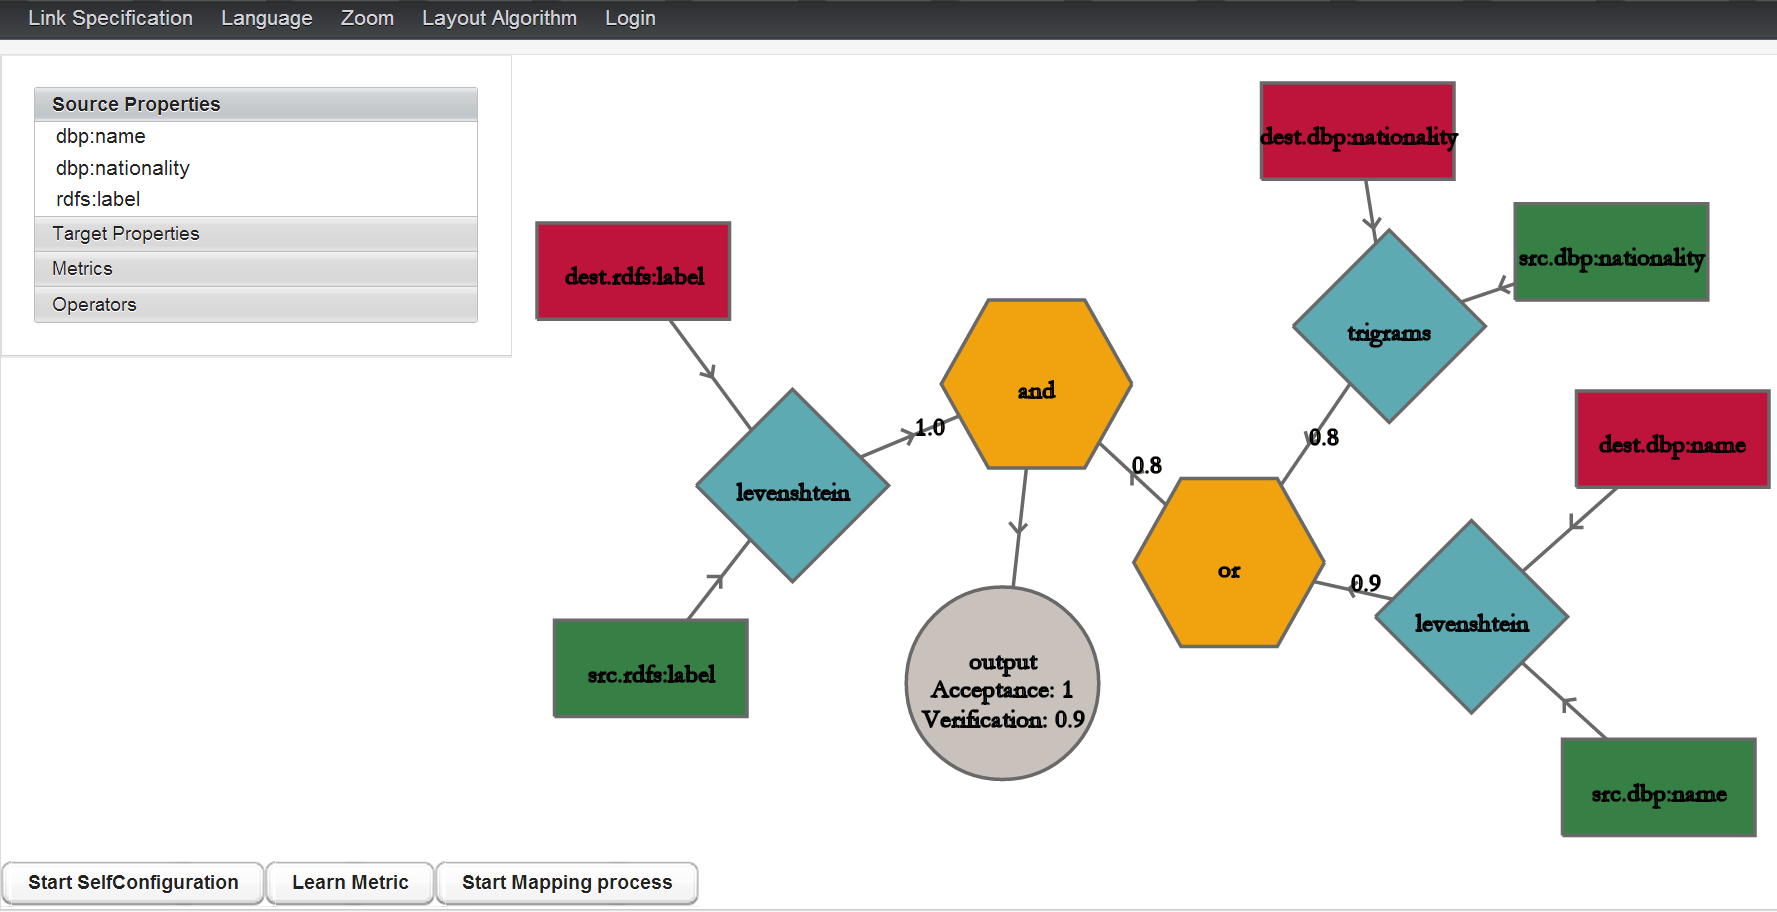
\includegraphics[width=0.7\textwidth]{images/saim_screenshot}
\caption{Screenshot of SAIM}
\label{fig:saim_screenshot}
\end{figure}

\subsection{Using Named Entity Recognition}
The geographical information hidden in datatype properties is retrieved by using Named Entity Recognition.
In the first version of \geolift, we rely on the FOX framework.
The FOX framework is a stateless and extensible framework that encompasses keyword extraction and named entity recognition. 
Its architecture consists of three layers as shown in Figure \ref{fig:foxArchitecture}.

\begin{figure}[htb]
\centering
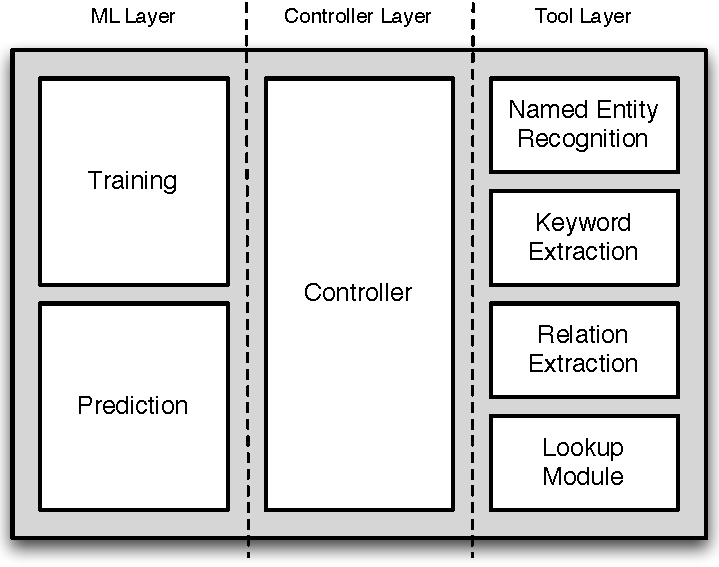
\includegraphics[width=0.55\textwidth]{images/FOX_Architecture}
\caption{Architecture of the FOX framework.}%
\label{fig:foxArchitecture}
\end{figure}

%The framework consists of three layers: a machine-learning layer, a controller layer and a tool layer.
FOX takes text or HTML as input.
Here we use the objects of datatype properties, i.e., plain text.
This data is sent to the \emph{controller layer}, which implements the functionality necessary to clean the data, i.e., remove HTML and XML tags as well as further noise.
Once the data has been cleaned, the controller layer begins with the orchestration of the tools in the \emph{tool layer}.
Each of the tools is assigned a thread from a thread pool, so as to maximize usage of multi-core CPUs.
Every thread runs its tool and generates an event once it has completed its computation.
In the event that a tool does not complete after a set time, the corresponding thread is terminated. 
So far, FOX integrates tools for KE, NER and RE. The KE is realized by tools such as KEA\footnote{\url{http://www.nzdl.org/Kea/}} and the Yahoo Term Extraction service\footnote{\url{http://developer.yahoo.com/search/content/V1/termExtraction.html}}.
In addition, FOX integrates the Stanford Named Entity Recognizer\footnote{\url{http://nlp.stanford.edu/software/CRF-NER.shtml}}~\cite{FIN+05}, the Illinois Named Entity Tagger\footnote{\url{http://cogcomp.cs.illinois.edu/page/software_view/4}}~\cite{RARO09} and Alchemy\footnote{\url{http://www.alchemyapi.com}} for NER. 

The results from the tool layer are forwarded to the \emph{prediction module} of the \emph{machine-learning layer}.
The role of the prediction module is to generate FOX's output based on the output the tools in FOX's backend.
For this purpose, it implements several ensemble learning techniques~\cite{DIE00} with which it can combine the output of several tools. 
Currently, the prediction module carries out this combination by using a feed-forward neural network. 
%say a bit about the first evaluation
The neural network inserted in FOX was trained by using 117 news articles. 
It reached 89.21\% F-Score in an evaluation based on a ten-fold-cross-validation on NER, therewith outperforming even commercial systems such as Alchemy.

Once the neural network has combined the output of the tool and generated a better prediction of the named entities, the output of FOX is generated by using the vocabularies shown in Figure \ref{fig:annotation-vocab}.
These vocabularies extend the two broadly used vocabularies Annotea\footnote{\url{http://www.w3.org/2000/10/annotation-ns#}} and Autotag~\footnote{\url{http://commontag.org/ns#}}. In particular, we added the constructs explicated in the following:
\begin{itemize}
    \item \texttt{scms:beginIndex} denotes the index in a literal value string at which a particular annotation or keyphrase begins;
    \item \texttt{scms:endIndex} stands for the index in a literal value string at which a particular annotation or keyphrase ends;
    \item \texttt{scms:means} marks the URI assigned to a named entity identified for an annotation;
    \item \texttt{scms:source} denotes the provenance of the annotation, i.\,e., the URI of the tool which computed the annotation or even the system ID of the person who curated or created the annotation and
		\item \texttt{scmsann} is the namespace for the annotation classes, i.e, location, person, organization and miscellaneous.
\end{itemize}

\begin{figure}[htb]
\centering
\subfloat[fig:ner][Named Entity Annotation]{
    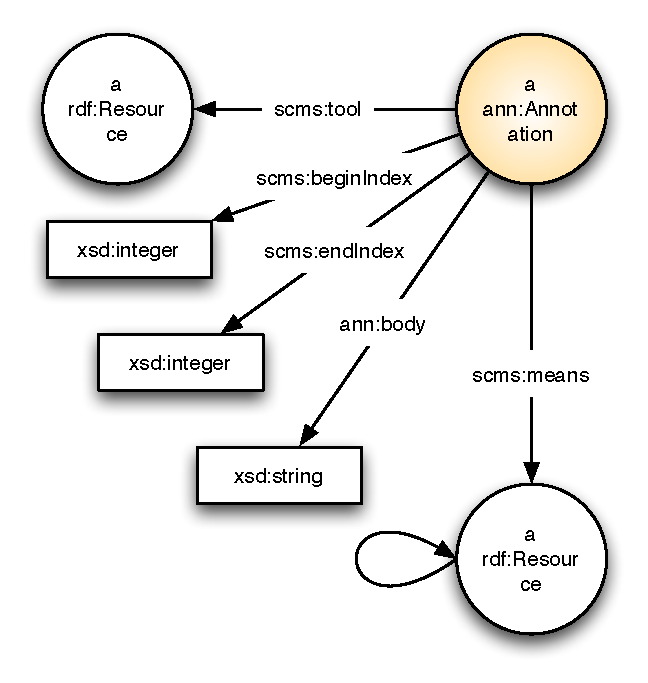
\includegraphics[scale=0.50]{images/NEAnnotation}
}\qquad
\subfloat[fig:ke][Keyword Annotation]{
    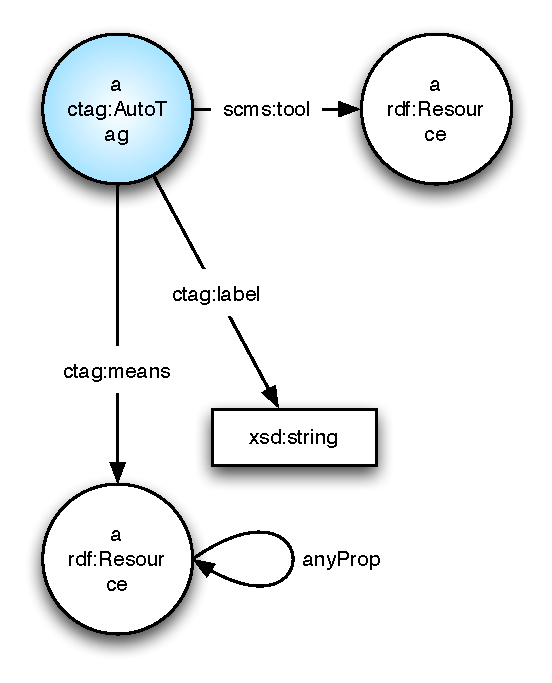
\includegraphics[scale=0.50]{images/KWAnnotation}
}
\caption{Vocabularies used by FOX for representing named entities (a) and keywords (b)}
\label{fig:annotation-vocab}
\end{figure}


\section{Developers' Manual}

\subsection{\geolift packages}
\geolift contains five basic \emph{Java} packages: 
\begin{enumerate}
 \item \texttt{IO package} which deals with input/output operations using:
   \begin{itemize}
    \item \texttt{Reader} class which handles all RDF reading process from file/URL/EndPoint. 
    \item \texttt{Writer} class which handles all the RDF writing process. 
  \end{itemize}

  \item\texttt{Modules package} contains the \texttt{GeoLiftModule} interface which is implemented by all modules' classes.
      All modules can be created using the \texttt{ModuleFactory} class calling its \texttt{createModule()} method with the desired module's name as parameter.
      Also, the \texttt{getImplementations()} method returns all implemented modules.
      Currently, five modules are implemented:
      \begin{itemize}
	\item \texttt{DereferencingModule} class which handles dereferencing  geographical information extending process. 
	\item \texttt{LinkingModule} class which handles linking geographical information extending processes. 
	\item \texttt{NLPModule} class which handles named entity extraction process.
	\item \texttt{AuthorityConformationModule} class which handles the subject authority conformation process.
	\item \texttt{PredicateConformationModule} class which handles the predicates conformation process.
	\item \texttt{FilterModule} class which handles filter process.
      \end{itemize}
  
   \item \texttt{Operators package} contains the \texttt{GeoLiftOperator} interface which is implemented by all operators' classes.
    All operators can be created using the \texttt{OperatorFactory} class calling its \texttt{createOperator()} method with the desired operator's name as parameter.
      \begin{itemize}
	\item \texttt{SplitOperator} class to generate from 1 input dataset a set of $n \geq 2$ clone output datasets.
	\item \texttt{MergeOperator} class to generate one merged output dataset out of $n \geq 2$ input datasets.
      \end{itemize}
 
  \item \texttt{Helper package} containing helper classes used by \geolift such as vocabularies classes.
  
  \item \texttt{Workflow package} containing classes responsible for \geolift overall execution process.
\end{enumerate}



\subsection{\geolift Modules}
    By \emph{Modules} we mean these artifacts in charge of generating geographical data based on RDF data. 
    % To this aim, they implement the three intuitions presented above.
    The input for such a module is an RDF dataset.
    The output is also an RDF dataset enriched with geographical information.
    Formally, a module can thus be regarded as a function $\mu: \mathcal{R} \rightarrow \mathcal{R}$, where $\mathcal{R}$ is the set of all RDF datasets.
    Currently, \geolift implements six modules: dereferencing, linking, NLP, authority conformation, predicate conformation and filter.

    All modules implement the \texttt{GeoLiftModule} interface methods 
    \begin{itemize}
      \item Model process() method takes as input a \emph{Jena} model and a Map of different parameters in form of \texttt{("parameterName", "parameterValue")},
    and as output all \geolift module generates a Jena model also, this organization ease the usage of the modules in different workflows.
      \item getParameters(), returns list of all available module parameters.
      \item getNecessaryParameters(), returns list of all necessary module parameters that have no default values.
      \item selfConfig(Model source, Model target), returns a map of parameters learned from the inputs (currently in progress).
    \end{itemize}

    Adding new modules to \geolift is possible by implementing the \texttt{GeoLiftModule}.
    \subsubsection{Dereferencing Module}

    For datasets which contain similarity proprieties links (e.g. \texttt{owl:sameAs}), we deference all links from the dataset to other datasets by using a content negotiation on HTTP as shown in Figure~\ref{fig:contentNegotiation}.
    This returns a set of triples that needs to be filtered for relevant geographical information.
    Here, we use a predefined list of attributes that links to geographical information.
    Amongst others, we look for \texttt{geo:lat}, \texttt{geo:long}, \texttt{geo:lat\_long}, \texttt{geo:line} and \texttt{geo:polygon}.
    The list of retrieved property values can be configured.

%     \subsubsection{Input}
%     \begin{itemize}
%     \item \texttt{Data model} contains the triples of the dataset to be enriched 
%     (This data model can be an output from previous stage or can be loaded from file/URI directly before using the module). 
%     \item \texttt{Predicates list} list of interested predicates to be added as enrichment to the data model.
%     Table \ref{tbl:derefPram} provides details about each of the \texttt{DereferencingModule} module's parameters.
%     \end{itemize}

    \begin{table}
    \caption{Dereferencing module parameters} \label{tbl:derefPram}
    \small
    \begin{tabularx}{\textwidth}{@{}lX@{}}
    % \begin{tabular}{@{}  l  l  l @{}}
    \toprule
    \textbf{Parameter Key} 		& \textbf{Parameter value}\\
    \toprule
    \texttt{inputProperty<n>} 	& List of interesting predicates to enrich the model, and their Objects' values. e.g.$\langle$``inputProperty1'',``\url{http://www.w3.org/2003/01/geo/wgs84_pos#lat}''$\rangle$. \textbf{Mandatory parameter}\\
    \midrule
    \texttt{outputProperty<n>} 	& The enriched output property. By default this parameter is set to \url{http://geoknow.org/ontology/relatedTo}\\
    \midrule
    \texttt{useBlankNodes}		& Use blank node in output dataset. By default, this parameter is set to \texttt{false}.\\
    \bottomrule
    % \end{tabular}
    \end{tabularx}
    \end{table}
    
%     \subsubsection{Output}
%     \begin{itemize}
%     \item \texttt{Data model} enriched data model with additional Geo-spatial information added by the given input predicates with its extracted object values.
%     \end{itemize}

%     \subsubsection{Process}
    In this module, a \emph{Java Jena} model and a list of interested predicates are given as inputs.
    This is done by iterating over the model's resources (dubbed as original resources) 
    and for each of the original resource an extraction of the predicates' values (objects) that are in the form of URI is performed. 
    These URIs (dubbed as dereferenced resources) are more filtered to be the resources used in \emph{DBpedia}.
    The dereferenced resources are handled by a dereference operation in order to find the interested predicates list for them.
    Such predicates and their objects' values are fetched and added to the the original resource to extend its information.
%     \subsubsection{Code Sample}
    Listing \ref{lst:DereferencingModule} provides a sample code showing how to use the \texttt{DereferencingModule} module:

    \begin{lstlisting}[label=lst:DereferencingModule, float=tp, numbers=left, numberstyle=\tiny, caption = Code fragment to call the \texttt{DereferencingModule} class.]
    // Define DereferencingModule object
    DereferencingModule u = ModuleFactory.createModule("dereferencing");
    // Define parameters Map
    Map<String, String> parameters = new HashMap<String, String>();
    // Set parameters
    parameters.put("predicate1", predicate1Value);
    parameters.put("predicate2", predicate2Value);
    // read input Model
    Model model = Reader.readModel(datasetSource);
    // Enrich the Model
    Model resultedModel = u.process(model, parameters);
    // Use the enriched model
    Writer.writeModel(enrichedModel, "TTL", System.out);
    \end{lstlisting}

    \subsubsection{Linking Module}
    Links to geographical resources do not occur in several knowledge bases.
    Here, we rely on the metrics implemented in the \limes framework\footnote{\url{http://limes.sf.net}}~\cite{NGAU11,NGON12c,NGO+13c} to link the resources in the input dataset with geographical datasets.
  
    \texttt{LinkingModule} have two inputs: an input model and list of parameters (see table~\ref{tbl:linkingPram} for parameters details).
    The linking process starts by generating links between the input dataset model and another dataset as second partner. 
    As said before, the linking process is done using \limes.
    \limes linking specification file is given as parameter.
%     By default, the links are stored in the \texttt{accept.nt} file.
    The output model of the \texttt{LinkingModule} is generated as the input model plus the generated links added with their original resources in the input model using    some linking property such as \texttt{owl:samAs}.
%     Another forward step is to feed the Dereference module with the resulted enriched model from Linking module as input. 
%     The previously generated links in the model in addition to other objects in the URIs form will be dereferenced adding more and detailed geographical information.
    Listing \ref{lst:Linking} provides a sample code showing how to use the Linking module.

    \begin{table}
    \caption{Linking module parameters} \label{tbl:linkingPram}
    \small
    \begin{tabularx}{\textwidth}{@{}lX@{}}
    % \begin{tabular}{@{}  l  l  l @{}}
    \toprule
    \textbf{Parameter key} 	&  \textbf{Parameter value}\\
    \toprule
    \texttt{specFile}	& The path to specification file used for linking process, the original dataset to be enriched must be on the source dataset , e.g. \url {linkingModuleData/linking/spec.xml}.\\
    \midrule
    \texttt{linksFile}	& The path to links file resulted from the linking process. This file's path is the same as the one specified in LIME's specifications file as output file, e.g. \url {linkingModuleData/linking/links.nt}.\\
    \midrule
    \texttt{linksPart} 	& Represents the original model's URI position as source/left or target/right in the linking specifications. Its value is either 'source' or 'target'.\\ 
    \bottomrule
    % \end{tabular}
    \end{tabularx}
    \end{table}

    
    
    \begingroup
	\fontsize{8pt}{10pt}\selectfont
    \begin{lstlisting}[label=lst:Linking, float=tp, numbers=left, numberstyle=\tiny, caption = Code fragment to call the \texttt{Linking} class.]
    // Define Linking object
    Linking l = ModuleFactory.createModule("linking");
    // Define parameters Map
    Map<String, String> parameters = new HashMap<String, String>();
    // Set parameters
    parameters.put("datasetSource",datasetSourceValue);
    parameters.put("specFilePath",specFilePathValue);
    parameters.put("linksFilePath",linksPathValue);
    parameters.put("linksPart",linksPartValue);
    // read input Model
    Model model = Reader.readModel(parameters.get("datasetSource"));
    // Enrich the Model
    model = l.process(model, parameters);
    // Use the enriched model
    Writer.writeModel(enrichedModel, "TTL", System.out);
    \end{lstlisting}
    \endgroup

    \subsubsection{NLP Module}
	The geographical information hidden in datatype properties is retrieved by using Named Entity Recognition (NER).
	\geolift - as an expandable modeller framework - can inject any NER framework to implement the \emph{NLP module}.
	In the current version of \geolift, we rely on the FOX framework. 

%     \subsubsection{Input}
%     \begin{itemize}
%     \item \texttt{Data model} contains the dataset to be enriched 
%     (This data model can be an output from previous module or can be loaded from file/URI directly before using the module). 
%     \item \texttt{Parameters list} that will be used during the process. The \texttt{getParameters()} method of the \texttt{NLPModule} class returns a list of parameters,
%     which can be set by the user to provide custom control of the \emph{Named entity extraction} provided by the implemented \emph{FOX framework}.
%     \end{itemize}
% 
%     \subsubsection{Output}
%     \begin{itemize}
%     \item \texttt{Data model} enriched with additional Geo-spatial information URIs represented by the \texttt{addedGeoProperty} predicates, 
%     witch by default is \texttt{gn:relatedTo\footnote{Prefix \texttt{gn} stands for \texttt{http://geoknow.org/ontology/}}} predicates.
%     \end{itemize}
% 
%     \subsubsection{Process}
%     The \texttt{process()} method of the \texttt{NLPModule} class takes as input a \emph{Jena} model and a \texttt{Map} of different parameters, 
%     and as output it generates a \emph{Jena} model also.
    Table \ref{tbl:nlpPram} provides details about the \texttt{NLPModule}'s parameters.
% 
%     \subsubsection{Code Sample}
    A sample code demonstrating the \texttt{NLPModule} class is provided introduced in Listing~\ref{lst:NLPModule}.

    \begin{table}
    \caption{NLP module parameters} \label{tbl:nlpPram}
    \small
    \begin{tabularx}{\textwidth}{@{}lX@{}}
    % \begin{tabular}{@{}  l  l  l @{}}
    \toprule
    \textbf{Parameter key} 	& \textbf{Parameter value} \\
    \toprule
    % \texttt{input} 		& The input file/URI to be enriched\\
    % \midrule
    % \texttt{output} 		& The output file to write the enriched model to it\\
    % \midrule
    \texttt{literalProperty}	& Literal property used by FOX for NER. If not set, the top ranked literal property will be pecked automatically by \texttt{LiteralPropertyRanker} sub-module, which ranks the  lateral properties of a model according to the average size of each literal property divided by the number of instances of such property.\\
    \midrule
    \texttt{addedGeoProperty}& property added to the input model with additional knowledge through NLP. By default, this parameter is set to \emph{gn:relatedTo\footnotemark[11]}\\
    \midrule
    \texttt{useFoxLight} 	& An implemented NER class name, either: 
			      \begin{itemize}
				  \itemsep-0.5em
				  \item \url{org.aksw.fox.nertools.NEROpenNLP}
				  \item \url{org.aksw.fox.nertools.NERIllinoisExtended}
				  \item \url{org.aksw.fox.nertools.NERIllinoisExtended}
				  \item \url{org.aksw.fox.nertools.NERBalie}
				  \item \url{org.aksw.fox.nertools.NERStanford}
			      \end{itemize}
			      By default this parameter is set to \url{OFF} in which all NER classes runs in parallel and a combined result will be returned, if this parameter is given with a wrong value, \url{org.aksw.fox.nertools.NERStanford} will be used. \\
    \midrule
    \texttt{NERType} 	& Force FOX to look for a specific NE's types only. Available types are: \texttt{location} (default value), \texttt{person},\texttt{organization}, and \texttt{all} to retrieve the all the previous three types.\\ 
    \midrule
    \texttt{askEndPoint} 	& Ask the \emph{DBpedia} endpoint for each location returned by FOX (setting it generates slower execution time but more accurate results). By default this parameter is set to \emph{false}\\
    \midrule
%     \texttt{foxType} 	&  text or an URL (e.g.: `G. W. Leibniz was born in Leipzig`, '\url{http://en.wikipedia.org/wiki/Leipzig_University}`). By default, this parameter is set to \emph{TEXT} \\
%     \midrule
%     \texttt{foxTask} 	& FOX task \texttt{:\{NER\}} for Named Entity RecognitionBy. By default, this parameter is set to \emph{NER}\\
%     \midrule
    % \texttt{foxInput} 	& FOX actual input as text or an URL default, this parameter is set to \emph{""}\\
    % \midrule
%     \texttt{foxOutput} 	& FOX output format: \{\texttt{ JSON-LD | N-Triples | RDF/\{ JSON | XML \}}\}. By default, this parameter is set to \emph{Turtle}\\
%     \midrule
%     \texttt{foxUseNif} 	& FOX generates NIF: \{ true $\rvert$ false \}. By default, this parameter is set to \emph{false}\\
%     \midrule
%     \texttt{foxReturnHtml} 	& FOX returns HTML: \texttt{\{ true $\rvert$ false \}}. By default, this parameter is set to \emph{false}\\ 
%     \bottomrule
    % \end{tabular}
    \end{tabularx}
    \end{table}

    \begin{lstlisting}[label=lst:NLPModule, float=tp, numbers=left, numberstyle=\tiny, caption = Code fragment to call the \texttt{NLPModule} class.]
    // Define NLPModule object
    NLPModule geoEnricher= ModuleFactory.createModule("nlp");
    // Define parameters Map
    Map<String, String> parameters = new HashMap<String, String>();
    // Set parameters
    parameters.put("useFoxLight", "OFF");
    parameters.put("askEndPoint", "false");
    // read input Model
    Model inputModel = Reader.readModel(inputFileValue);
    // Enrich the Model
    Model enrichedModel = geoEnricher.process(inputModel, parameters);
    // Use the enriched model
    Writer.writeModel(enrichedModel, "TTL", System.out);
    \end{lstlisting}
    

\subsubsection{Authority Conformation Module}
    Change a specified source URI authority to a specified target URI authority.
    For example, using source URI authority of \url{http://dbpedia.org} and target URI authority of \url{http://deer.org} changes a resource like \url{http://dbpedia.org/Berlin} to \url{http://deer.org/Berlin}.
    As an example, listing~\ref{lst:aConf} introduces a code segment to manipulate the \texttt{AuthorityConformationModule} to change the source authority from \url{http://dbpedia.org} to the target authority \url{http://deer.org/Berlin}.
    Table~\ref{tbl:aConf} provides a full list of the authority conformation module parameters.
    
    \begin{table}
      \caption{Conformation module parameters} \label{tbl:aConf}
      \small
	\begin{tabularx}{\textwidth}{@{}lX@{}}
	    % \begin{tabular}{@{}  l  l  l @{}}
	    \toprule
	    \textbf{Parameter key} 	& \textbf{Parameter value} \\
	    \toprule
	    \texttt{sourceSubjectAuthority}	& Source URI to be replaced.\\
	    \midrule
	    \texttt{targetSubjectAuthority}	& Target URI to replace the sourceURI.\\
	    \bottomrule
	    % \end{tabular}
	\end{tabularx}
    \end{table}.
    
\subsubsection{Predicate Conformation Module}
    The \texttt{PredicateConformationModule} can be used to change a specific source properties to specific target properties.
    As an example, listing~\ref{lst:pConf} introduces a code segment to manipulate the \texttt{PredicateConformationModule} that changes all occurrences of \texttt{RDF:label} to \texttt{SKOS:prefLabel}.
    Table~\ref{tbl:pConf} provides a full list of the predicate conformation module parameters.
    

    \begin{table}
    \caption{Conformation module parameters} \label{tbl:pConf}
    \small
    \begin{tabularx}{\textwidth}{@{}lX@{}}
    % \begin{tabular}{@{}  l  l  l @{}}
    \toprule
    \texttt{sourceProperty<i>}	& $i^{th}$ source property to be replaced by the $i^{th}$ target property.\\
    \midrule
    \texttt{targetProperty<i>}	& $i^{th}$ target property to replace the $i^{th}$ source property.\\
    \bottomrule
    % \end{tabular}
    \end{tabularx}
    \end{table}.
    
    \begin{lstlisting}[label=lst:aConf, float=tp, numbers=left, numberstyle=\tiny, caption = Code fragment to call the \texttt{AuthorityConformationModule} class.]
    // Define NLPModule object
    AuthorityConformationModule geoEnricher = ModuleFactory.createModule("authorityconformation");
    // Define parameters Map
    Map<String, String> parameters = new HashMap<String, String>();
    // Set parameters
    parameters.put("sourceSubjectAuthority", "http://dbpedia.org");
    parameters.put("targetSubjectAuthority", "http://deer.org");
    // read input Model
    Model inputModel = Reader.readModel(inputFileValue);
    // Enrich the Model
    Model enrichedModel = geoEnricher.process(inputModel, parameters);
    // Use the enriched model
    Writer.writeModel(enrichedModel, "TTL", System.out);
    \end{lstlisting}
    
        \begin{lstlisting}[label=lst:pConf, float=tp, numbers=left, numberstyle=\tiny, caption = Code fragment to call the \texttt{PredicateConformationModule} class.]
    // Define NLPModule object
    PredicateConformationModule geoEnricher = ModuleFactory.createModule("predicateconformation");
    // Define parameters Map
    Map<String, String> parameters = new HashMap<String, String>();
    // Set parameters
    parameters.put("sourceProperty1", "http://www.w3.org/1999/02/22-rdf-syntax-ns#label");
    parameters.put("targetProperty1", "http://www.w3.org/2004/02/skos/core#prefLabel");
    // read input Model
    Model inputModel = Reader.readModel(inputFileValue);
    // Enrich the Model
    Model enrichedModel = geoEnricher.process(inputModel, parameters);
    // Use the enriched model
    Writer.writeModel(enrichedModel, "TTL", System.out);
    \end{lstlisting}

\subsubsection{Filter Module}
    Runs a set of triples patterns' against an input model to filter some triples out of it and export them to an output model. 
    For example running triple pattern \texttt{"?s \url{<http://dbpedia.org/ontology/abstract>} ?o"} against an input model containing "\url{http://dbpedia.org/resource/Berlin}" will generate output model containing only Berlin's abstracts of \emph{DBpedia}.
    Listing~\ref{lst:filterModule} demonstrate the filter module usage.
    table \ref{tbl:filterPram} provides a full list of the filter module parameters.

    \begin{table}
    \caption{Filter module parameters} \label{tbl:filterPram}
    \small
    \begin{tabularx}{\textwidth}{@{}lX@{}}
    % \begin{tabular}{@{}  l  l  l @{}}
    \toprule
    \textbf{Parameter key} 	& \textbf{Parameter value} \\
    \toprule
    \texttt{triplesPattern}	& Set of triple pattern to run against the input model of the filter module. By default, this parameter is set to \texttt{?s ?p ?o.} which generate the whole input model as output, changing the values of \texttt{?s}, \texttt{?p} and/or \texttt{?o} will restrict the output model.\\
    \bottomrule
    % \end{tabular}
    \end{tabularx}
    \end{table}
    
    \begin{lstlisting}[label=lst:filterModule, float=tp, numbers=left, numberstyle=\tiny, caption = Code fragment to call the \texttt{FilterModule} class.]
    // Define NLPModule object
    FilterModule geoEnricher= ModuleFactory.createModule("filter");
    // Define parameters Map
    Map<String, String> parameters = new HashMap<String, String>();
    // Set parameters
    parameters.put("triplesPattern ", "?s <http://dbpedia.org/ontology/abstract> ?o");
    parameters.put("askEndPoint", "false");
    // read input Model
    Model inputModel = Reader.readModel(inputFileValue);
    // Enrich the Model
    Model enrichedModel = geoEnricher.process(inputModel, parameters);
    // Use the enriched model
    Writer.writeModel(enrichedModel, "TTL", System.out);
    \end{lstlisting}
    
\subsection{\geolift Operators}
The idea behind operators is to enable users to define a workflow for processing their input dataset. 
\geolift operators combine the enrichment modules and allow defining a workflow for processing information.
Note that the format of the input and output of operator is identical. 
Thus, the user is empowered to create workflows of arbitrary complexity by simply connecting modules and/or operators.
Formally, an operator can be regarded as a function $\varphi: \mathcal{R}^* \rightarrow \mathcal{R}^*$.

  All operators classes implement the \texttt{GeoLiftOperator} interface's two methods \texttt{getParameters()} and \texttt{process()},
 where the \texttt{getParameters()} method returns a list of its module input parameters,
 and the \texttt{process()} method takes as input a list of \emph{Jena} models and a \emph{Map} of different parameters in form of \texttt{("parameterName", "parameterValue")}.
 Each of the \geolift operators outputs a list of Jena models.
 This organization ease the usage of the operators in different workflows.
 Adding new operators to \geolift is possible by implementing the \texttt{GeoLiftOperator}.

\subsubsection{Split Operator}
The idea behind the split operator is to enable parallel execution of different modules in the same dataset. 
The split operator takes one dataset as input and produces $n \geq 2$ output datasets, which are all identical to the input dataset.
Each of the output datasets of the split operator has its own workflow (as to be input to any other module or operator).
Thus, \geolift is able to execute all workflows of output datasets in parallel. 

\subsubsection{Merge Operator}
The idea behind the merge operator is to enable combining datasets.
The merge operator takes a set of $n \geq 2$ input datasets and merges them into one output dataset containing all the input datasets' triples.
As in case of split operator, the merged output dataset has its own workflow (as to be input to any other module or operator).

\section{\geolift RDF Specification Paradigm}
In the current version of \geolift we introduce our new RDF based specification paradigm.
The main idea behind this new paradigm is to enable the processing execution of specifications in an efficient way.
To this end, we first decided to use RDF as language for the specification. This has the main advantage of allowing for creating specification repositories which can be queried easily with the aim of retrieving accurate specifications for the use cases at hand. Moreover, extensions of the specification language do not require a change of the specification language due to the intrinsic extensibility of ontologies. The third reason for choosing RDF as language for specifications is that we can easily check the specification for correctness by using a reasoner, as the specification ontology allows for specifying the restrictions that specifications must abide by.

% listing~\ref{lst:rdfconf} 
introduces an example of RDF specification file presented in turtle serialization, which will be used as a guiding example through the next subsections.
For the sake of  clarity, we represent the configuration file in form of graph in figure~\ref{fig:rdfconf}.


\subsection{\geolift Execution Workflow}
First of all, \geolift determines the set of output datasets $D = \{d_1, \dots , d_n\}$, 
i.e. datasets which are included as output of some modules/operators but not as input to any other modules/operators.
In our example it is only $d_8$.
Then, for each dataset $d_i$ in $D$, \geolift tries to find $d_i$ either trivially from file/URI/endpoint or recursively by solving for modules/operators that generate $d_i$ as output.

Going back to our example, \geolift first tries to read $d_8$ trivially but it fail as there is no direct way to read it. 
Then, \geolift recursively goes for solving the \texttt{Conformation module} as it generates $d_8$ as output. 
This recursive procedure continues until \geolift reads the dataset $d_1$ from the endpoint.
Afterwards, going back in the recursion stack \geolift produces the triples of $d_8$.

\subsubsection{RDF Specification Resources} 

\geolift RDF specification file may contain four main resource types (dataset, module, operator and parameter). 
in the following we will describe each of them along with our example shown in listing~\ref{lst:rdfconf}. 

% \todo[inline]{There is a problem inserting a lstlisting in this file (I an tired of trying to fix), @Axel Can u please try to fix this?}

\begin{lstlisting}[label=lst:rdfconf, float=tp, basicstyle=\scriptsize, numbers=left, numberstyle=\tiny, caption = Example of RDF configuration file.]
@prefix : <http://geoknow.org/specsontology/> .
@prefix rdfs: <http://www.w3.org/2000/01/rdf-schema#> .
@prefix geo: <http://www.w3.org/2003/01/geo/wgs84_pos#> .
:d1		a		:Dataset ;
		:hasUri		<http://dbpedia.org/resource/Berlin> ;
		:fromEndPoint	<http://dbpedia.org/sparql> .
:d2		a		:Dataset .
:d3		a		:Dataset .
:d4		a		:Dataset .
:d5		a		:Dataset .
:d6		a		:Dataset .
:d7		a		:Dataset .
:d8		a		:Dataset ;
		:outputFile	"GeoLiftBerlin.ttl" ;
		:outputFormat	"Turtle" .
:deref		a		:Module, :DereferencingModule  ;
		rdfs:label	"Dereferencing module" ;
		:hasInput	:d1 ;
		:hasOutput	:d2 ;
		:hasParameter	:derefParam1 .
:derefParam1	a   :ModuleParameter, :DereferencingModuleParameter ;
		:hasKey		"inputProperty1" ;
		:hasValue	geo:lat .
:split		a		:Operator, :SplitOperator  ;
		rdfs:label	"Split operator" ;
		:hasInput	:d2 ;
		:hasOutput	:d3, :d4 .
:nlp		a		:Module, :NLPModule  ;
		rdfs:label	"NLP module" ;
		:hasInput	:d3 ;
		:hasOutput	:d5 ;
		:hasParameter	:nlpPram1, :nlpPram2 .
:nlpPram1	a		:ModuleParameter, :NLPModuleParameter ;
		:hasKey		"useFoxLight" ;
		:hasValue	"OFF" .
:nlpPram2 	a		:ModuleParameter, :NLPModuleParameter ;
		:hasKey		"askEndPoint" ;
		:hasValue	false .
:filter		a		:Module, :FilterModule  ;
		rdfs:label	"Filter module" ;
		:hasInput	:d4 ;
		:hasOutput	:d6 ;
		:hasParameter	:FilterPram1 .
:filterPram1	a      :ModuleParameter, :NLPModuleParameter ;
	    :hasKey    "triplesPattern" ;
	    :hasValue "?s <http://dbpedia.org/ontology/abstract> ?o".
:merge		a		:Operator, :MergeOperator  ;
		rdfs:label	"Merge operator" ;
		:hasInput	:d6, :d5 ;
		:hasOutput	:d7 .
:aconform	a	:Module, :AuthorityConformationModule  ;
		rdfs:label	"Authority Conformation module" ;
		:hasInput	:d7 ;
		:hasOutput	:d8 ;
		:hasParameter	:aconformPram1, :aconformPram2 .
:aconformPram1	a		:ModuleParameter, :NLPModuleParameter ;
		:hasKey		"sourceSubjectAuthority" ;
		:hasValue	"http://dbpedia.org" .
:aconformPram2	a		:ModuleParameter, :NLPModuleParameter ;
		:hasKey		"targetSubjectAuthority" ;
		:hasValue	"http://deer.org" .
\end{lstlisting}


\begin{itemize}
 \item \textbf{Dataset Resource}
    As its name implies, a Dataset resource represents a dataset. 
    For an example see~listing~\ref{lst:rdfconf}~(lines 4:6), in which the RDF specification represents a dataset with URI \texttt{\url{http://dbpedia.org/resource/Berlin}} and endpoint \texttt{\url{http://dbpedia.org/sparql}}.
    \geolift extracts the CBD of the \emph{Berlin} resource from \emph{DBpedia} endpoint. 

    Beside defining a resource as a dataset (e.g.~listing~listing~\ref{lst:rdfconf}~(lines 4)),
    a dataset resource may also contain the following predicates:
    \begin{itemize}
	\item \texttt{rdfs:label} setting label for the dataset.
	\item \texttt{:hasUri} setting URI of the dataset resource, to read resource through content negotiation \emph{(e.g.~listing~listing~\ref{lst:rdfconf}~(line 5))}.
	\item \texttt{:fromEndPoint} end point to read the CBD from. 
	\emph{Note: must be used in conjunction with \texttt{:hasUri} predicate, otherwise an error will be generated by \geolift.} \emph{(e.g.~listing~\ref{lst:rdfconf}~(line 6))}.
	\item \texttt{:inputFile} input file to load the dataset from.
	\item \texttt{:outputFile} output file to save the dataset to \emph{(e.g.~listing~\ref{lst:rdfconf}~(lines 14))}.
	\item \texttt{:outputFormat} output format to save the dataset in it \emph{(e.g.~listing~\ref{lst:rdfconf}~(lines 14))}, Turtle format will be used as default format if this property is not set.
    \end{itemize}

  \item \textbf{Module Resource}
    Beside defining a resource as a module \emph{(e.g.~listing~\ref{lst:rdfconf}~(line 16))},
    a Module resource may also contain the following predicates:
    \begin{itemize}
	\item \texttt{rdfs:label} setting label for the module \emph{(e.g.~listing~\ref{lst:rdfconf}~(line 17))}.
	\item \texttt{:hasInput} setting input datasets for the module \emph{(e.g.~listing~\ref{lst:rdfconf}~(line 18))}.
	\item \texttt{:hasOutput} setting output datasets for the module \emph{(e.g.~listing~\ref{lst:rdfconf}~(line 19))}.
	\item \texttt{:hasParameter} setting parameters for the module \emph{(e.g. ~listing~\ref{lst:rdfconf}~(line 20))}.
    \end{itemize}

  \item \textbf{Operator Resource}
    Beside defining a resource as an operator \emph{(e.g.~listing~\ref{lst:rdfconf}~(line 24))},
    a Module resource may also contain the following predicates:
    \begin{itemize}
	\item \texttt{rdfs:label} setting a label for the operator \emph{(e.g.~listing~\ref{lst:rdfconf}~(line 25))}.
	\item \texttt{:hasInput} setting input datasets for the operator \emph{(e.g.~listing~\ref{lst:rdfconf}~(line 26))}.
	\item \texttt{:hasOutput} setting output datasets for the operator \emph{(e.g.~listing~\ref{lst:rdfconf}~(line 27))}.
	\item \texttt{:hasParameter} setting parameters for the operator.
    \end{itemize}

  \item \textbf{Parameter Resource}
    Beside defining a resource as a parameter \emph{(e.g.~listing~\ref{lst:rdfconf}~(line 21))},
    a Module resource may also contain the following predicates:
    \begin{itemize}
	\item \texttt{rdfs:label} setting label for the parameter.
	\item \texttt{:hasKey} setting the parameter key \emph{(e.g.~listing~\ref{lst:rdfconf}~(line 22))}.
	\item \texttt{:HasValue} setting the parameter value \emph{(e.g.~listing~\ref{lst:rdfconf}~(lines 23))}.
    \end{itemize}
    The values of (key, values) pairs are modules/operators dependent    \footnote{For more details about (key, values) pairs of each  module/operator, see \geolift user manual at  \url{https://github.com/GeoKnow/GeoLift/blob/master/GeoLiftManual/GeoLiftManual.pdf}}.
    
\end{itemize}
\begin{figure}
\centering
  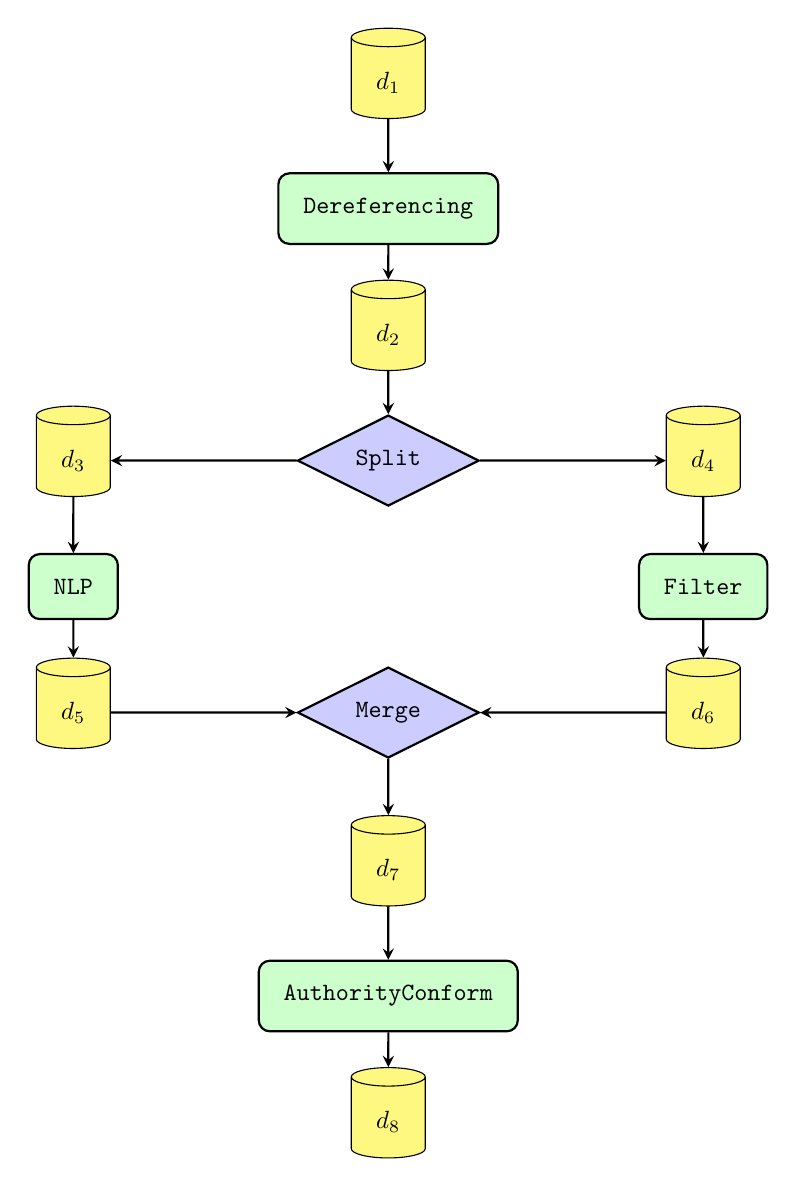
\begin{tikzpicture}[scale = 0.8, every node/.style={scale=0.9}, >=stealth, node distance=3cm, 
      database/.style={cylinder, cylinder uses custom fill, cylinder body fill=yellow!50, cylinder end fill=yellow!50, shape border rotate=90, aspect=0.25, inner sep=10pt, draw},
      operator/.style={draw=black,fill=blue!20,thick,inner sep=5pt, diamond, aspect=2, draw},
      module/.style={draw=black,fill=green!20,thick,rounded corners,inner sep=10pt, draw},
      parameter/.style={draw=gray,fill=gray!20,thick,rounded corners,inner sep=10pt, draw}]
      \node[database] (d1) at (15,5) {\textbf{$d_1$}};
      \node (deref)  at (15,3) [module] {\texttt{Dereferencing}};
      \draw[thick,->] (d1) -- (deref);
%       \node (derefParam1)  at (23,3)  {\texttt{geo:lat}};
%       \draw[->,thin] (deref) to node[ rectangle, draw, fill=white,draw=white]{$inputProperty1$} (derefParam1);
      \node[database] (d2) at (15,1) {\textbf{$d_2$}};
      \node (split)  at (15,-1) [operator] {\texttt{Split}};
      \draw[thick,->] (deref) -- (d2);
      \draw[thick,->] (d2) -- (split);
      \node[database] (d3) at (10,-1) {\textbf{$d_3$}};
      \draw[thick,->] (split) -- (d3);
      \node (nlpleft)  at (10,-3) [module] {\texttt{NLP}};
      \draw[thick,->] (d3) -- (nlpleft);
      \node[database] (d4) at (20,-1) {\textbf{$d_4$}};
      \draw[thick,->] (split) -- (d4);
      \node (filter)  at (20,-3) [module] {\texttt{Filter}};
      \draw[thick,->] (d4) -- (filter);
      \node[database] (d5) at (10,-5) {\textbf{$d_5$}};
      \draw[thick,->] (nlpleft) -- (d5);
      \node[database] (d6) at (20,-5) {\textbf{$d_6$}};
      \draw[thick,->] (filter) -- (d6);
      \node (merge)  at (15,-5) [operator] {\texttt{Merge}};
      \draw[thick,->] (d5) -- (merge);
      \draw[thick,->] (d6) -- (merge);
      \node[database] (d7) at (15,-7.5) {\textbf{$d_7$}};
      \draw[thick,->] (merge) -- (d7);
      \node (AuthorityConform)  at (15,-9.5) [module] {\texttt{AuthorityConform}};
      \draw[thick,->] (d7) -- (AuthorityConform);
      \node[database] (d8) at (15,-11.5) {\textbf{$d_8$}};
      \draw[thick,->] (AuthorityConform) -- (d8);
  \end{tikzpicture}
  \caption{Graph representation of configuration file presented by listing~\ref{lst:rdfconf}}
  \label{fig:rdfconf}
\end{figure}

% Listing~listing~\ref{lst:rdfconf} introduces an example of RDF configuration file, to make it easier to be understood we represent the configuration file in form of graph in figure~\ref{fig:rdfconf}.
% 
% \subsection{How \geolift execute the RDF configuration file?}
% First of all \geolift RDF configuration reader determines the set of output datasets $D$, 
% i.e. datasets which are included as output of some modules/operators but not as input to any other modules/operators.
% In our example it will be only $d_8$.
% 
% For each dataset in $D$ \geolift tries to find it either trivially from file, URI or endpoint if provided by the dataset node in the RDF configuration file, 
% or recursively buy solving for modules/operators that generate it as output.
% 
% Going beck to our example, \geolift first tries to read $d_8$ trivially but it fail as there are no direct way to get it. 
% Then, \geolift recursively go for solving the \texttt{Conformation} module as it generate $d_8$ as output. 
% This recursive procedure continues until it reads the dataset $d_1$ from the endpoint, then going back in the recursion stack.
% 
% \subsection{RDF Configuration main resources types}
% \geolift RDF configuration contains four main resource types (dataset, module, operator and parameter).
% 
% \subsubsection{Dataset Resource}
%     As it name implies, a Dataset resource represent a dataset. 
%     For an example see figure~listing~\ref{lst:rdfconf}(lines 4:6), in which it represent a dataset with URI \texttt{\url{http://dbpedia.org/resource/Berlin}} and endpoint \texttt{\url{http://dbpedia.org/sparql}}.
%     \geolift will generate the Concise Bounded Description (CBD)\footnote{For more details about CBD see \url{http://www.w3.org/Submission/CBD/}} of the \emph{Berlin} resource from \emph{DBpedia} endpoint. 
% 
%     Beside defining a resource as a dataset (e.g. figure~listing~\ref{lst:rdfconf}~(lines 4)),
%     a dataset resource may also contains the following predicates:
%     \begin{itemize}
% 	\item \texttt{rdfs:label} setting label for the dataset.
% 	\item \texttt{:hasUri} setting URI of the dataset resource, to read resource through content negotiation \emph{(e.g. figure~listing~\ref{lst:rdfconf}~(line 5))}.
% 	\item \texttt{:FromEndPoint} end point to read the CBD from. 
% 	\emph{Note: must be used in conjunction with \texttt{:hasUri} predicate, otherwise an error will be generated by \geolift.} \emph{(e.g. figure~listing~\ref{lst:rdfconf}~(line 6))}.
% 	\item \texttt{:inputFile} input file to load the dataset from.
% 	\item \texttt{:outputFile} output file to save the dataset to \emph{(e.g. figure~listing~\ref{lst:rdfconf}~(lines 14))}.
% 	\item \texttt{:outputFormat} output format to save the dataset in it \emph{(e.g. figure~listing~\ref{lst:rdfconf}~(lines 14))}, Turtle format will be used as default format if this property is not set.
%     \end{itemize}
% 
% \subsubsection{Module Resource}
%     Beside defining a resource as a module \emph{(e.g. figure~listing~\ref{lst:rdfconf}~(line 16))},
%     a Module resource may also contains the following predicates:
%     \begin{itemize}
% 	\item \texttt{rdfs:label} setting label for the module \emph{(e.g. figure~listing~\ref{lst:rdfconf}~(line 17))}.
% 	\item \texttt{:hasInput} setting input datasets for the module \emph{(e.g. figure~listing~\ref{lst:rdfconf}~(line 18))}.
% 	\item \texttt{:hasOutput} setting output datasets for the module \emph{(e.g. figure~listing~\ref{lst:rdfconf}~(line 19))}.
% 	\item \texttt{:hasParameter} setting parameters for the module \emph{(e.g. figure~listing~\ref{lst:rdfconf}~(line 20))}.
%     \end{itemize}
% 
% \subsubsection{Operator Resource}
%     Beside defining a resource as an operator \emph{(e.g. figure~listing~\ref{lst:rdfconf}~(line 24))},
%     a Module resource may also contains the following predicates:
%     \begin{itemize}
% 	\item \texttt{rdfs:label} setting a label for the operator \emph{(e.g. figure~listing~\ref{lst:rdfconf}~(line 25))}.
% 	\item \texttt{:hasInput} setting input datasets for the operator \emph{(e.g. figure~listing~\ref{lst:rdfconf}~(line 26))}.
% 	\item \texttt{:hasOutput} setting output datasets for the operator \emph{(e.g. figure~listing~\ref{lst:rdfconf}~(line 27))}.
% 	\item \texttt{:hasParameter} setting parameters for the operator.
%     \end{itemize}
% 
% \subsubsection{Parameter Resource}
%     Beside defining a resource as a parameter \emph{(e.g. figure~listing~\ref{lst:rdfconf}~(line 21))},
%     a Module resource may also contains the following predicates:
%     \begin{itemize}
% 	\item \texttt{rdfs:label} setting label for the parameter.
% 	\item \texttt{:hasKey} setting the parameter key \emph{(e.g. figure~listing~\ref{lst:rdfconf}~(line 22))}.
% 	\item \texttt{:HasValue} setting the parameter value \emph{(e.g. figure~listing~\ref{lst:rdfconf}~(lines 23))}.
%     \end{itemize}
%     The values of (key, values) pairs are modules/operators dependent.
%     see	modules/operators sections for more details.
% 
%     
% \begin{lstlisting}[label=lst:rdfconf, numbers=left, numberstyle=\tiny, caption = Example of RDF configuration file.]
% @prefix : <http://geoknow.org/specsontology/> .
% @prefix rdfs: <http://www.w3.org/2000/01/rdf-schema#> .
% @prefix geo: <http://www.w3.org/2003/01/geo/wgs84_pos#> .
% :d1		a		:Dataset ;
% 		:hasUri		<http://dbpedia.org/resource/Berlin> ;
% 		:FromEndPoint	<http://dbpedia.org/sparql> .
% :d2		a		:Dataset .
% :d3		a		:Dataset .
% :d4		a		:Dataset .
% :d5		a		:Dataset .
% :d6		a		:Dataset .
% :d7		a		:Dataset .
% :d8		a		:Dataset ;
% 		:outputFile	"GeoLiftBerlin.ttl" ;
% 		:outputFormat	"Turtle" .
% :deref		a		:Module, :DereferencingModule  ;
% 		rdfs:label	"Dereferencing module" ;
% 		:hasInput	:d1 ;
% 		:hasOutput	:d2 ;
% 		:hasParameter	:derefParam1 .
% :derefParam1	a   :ModuleParameter, :DereferencingModuleParameter ;
% 		:hasKey		"inputProperty1" ;
% 		:hasValue	geo:lat .
% :split		a		:Operator, :SplitOperator  ;
% 		rdfs:label	"Split operator" ;
% 		:hasInput	:d2 ;
% 		:hasOutput	:d3, :d4 .
% :nlp		a		:Module, :NLPModule  ;
% 		rdfs:label	"NLP module" ;
% 		:hasInput	:d3 ;
% 		:hasOutput	:d5 ;
% 		:hasParameter	:nlpPram1, :nlpPram2 .
% :nlpPram1	a		:ModuleParameter, :NLPModuleParameter ;
% 		:hasKey		"useFoxLight" ;
% 		:hasValue	"OFF" .
% :nlpPram2 	a		:ModuleParameter, :NLPModuleParameter ;
% 		:hasKey		"askEndPoint" ;
% 		:hasValue	false .
% :filter		a		:Module, :FilterModule  ;
% 		rdfs:label	"Filter module" ;
% 		:hasInput	:d4 ;
% 		:hasOutput	:d6 ;
% 		:hasParameter	:FilterPram1 .
% :filterPram1	a      :ModuleParameter, :NLPModuleParameter ;
% 	    :hasKey    "triplesPattern" ;
% 	    :hasValue "?s <http://dbpedia.org/ontology/abstract> ?o".
% :merge		a		:Operator, :MergeOperator  ;
% 		rdfs:label	"Merge operator" ;
% 		:hasInput	:d6, :d5 ;
% 		:hasOutput	:d7 .
% :conform	a			:Module, :ConformationModule  ;
% 		rdfs:label	"Conformation module" ;
% 		:hasInput	:d7 ;
% 		:hasOutput	:d8 ;
% 		:hasParameter	:conformPram1, :conformPram2 .
% :conformPram1	a		:ModuleParameter, :NLPModuleParameter ;
% 		:hasKey		"sourceURI" ;
% 		:hasValue	"http://dbpedia.org" .
% :conformPram2	a		:ModuleParameter, :NLPModuleParameter ;
% 		:hasKey		"targetURI" ;
% 		:hasValue	"http://geolift.org" .
% \end{lstlisting}
% 
% 
% \begin{figure}[!h]
% \centering
%   \begin{tikzpicture}[scale = 0.8, every node/.style={scale=0.9}, >=stealth, node distance=3cm, 
%       database/.style={cylinder, cylinder uses custom fill, cylinder body fill=yellow!50, cylinder end fill=yellow!50, shape border rotate=90, aspect=0.25, inner sep=10pt, draw},
%       operator/.style={draw=black,fill=blue!20,thick,inner sep=5pt, diamond, aspect=2, draw},
%       module/.style={draw=black,fill=green!20,thick,rounded corners,inner sep=10pt, draw},
%       parameter/.style={draw=gray,fill=gray!20,thick,rounded corners,inner sep=10pt, draw}]
%       \node[database] (d1) at (15,5) {\textbf{$d_1$}};
%       \node (deref)  at (15,3) [module] {\texttt{Dereferencing}};
%       \draw[thick,->] (d1) -- (deref);
% %       \node (derefParam1)  at (23,3)  {\texttt{geo:lat}};
% %       \draw[->,thin] (deref) to node[ rectangle, draw, fill=white,draw=white]{$inputProperty1$} (derefParam1);
%       \node[database] (d2) at (15,1) {\textbf{$d_2$}};
%       \node (split)  at (15,-1) [operator] {\texttt{Split}};
%       \draw[thick,->] (deref) -- (d2);
%       \draw[thick,->] (d2) -- (split);
%       \node[database] (d3) at (10,-1) {\textbf{$d_3$}};
%       \draw[thick,->] (split) -- (d3);
%       \node (nlpleft)  at (10,-3) [module] {\texttt{NLP}};
%       \draw[thick,->] (d3) -- (nlpleft);
%       \node[database] (d4) at (20,-1) {\textbf{$d_4$}};
%       \draw[thick,->] (split) -- (d4);
%       \node (filter)  at (20,-3) [module] {\texttt{Filter}};
%       \draw[thick,->] (d4) -- (filter);
%       \node[database] (d5) at (10,-5) {\textbf{$d_5$}};
%       \draw[thick,->] (nlpleft) -- (d5);
%       \node[database] (d6) at (20,-5) {\textbf{$d_6$}};
%       \draw[thick,->] (filter) -- (d6);
%       \node (merge)  at (15,-5) [operator] {\texttt{Merge}};
%       \draw[thick,->] (d5) -- (merge);
%       \draw[thick,->] (d6) -- (merge);
%       \node[database] (d7) at (15,-7.5) {\textbf{$d_7$}};
%       \draw[thick,->] (merge) -- (d7);
%       \node (conform)  at (15,-9.5) [module] {\texttt{Conformation}};
%       \draw[thick,->] (d7) -- (conform);
%       \node[database] (d8) at (15,-11.5) {\textbf{$d_8$}};
%       \draw[thick,->] (conform) -- (d8);
%   \end{tikzpicture}
%   \caption{Graph representation of configuration file presented by listing~\ref{lst:rdfconf}}
%   \label{fig:rdfconf}
% \end{figure}

% \textbf{Details of RDF configuration file will be here soon}
% Command-line execution of \geolift enable user-defined workflow of different modules using configuration file.
% Through the configuration file user can give different parameters to different modules.
% Currently, simple tab-separated values file format is implemented as configuration file, 
% where values are set in form of \texttt{(executionModelIndex moduleName moduleParameterName moduleParameterVale)}.
% 
% The \texttt{executionModelIndex} is just an index starts with one and repeats for all \texttt{moduleParameterName moduleParameterVale} pairs for the same \texttt{moduleName}.
% listing \ref{lst:geoliftConfig} provides a example of a configuration file to run four modules.
% Note that the third and the forth module have the same \texttt{moduleName}, but using the \texttt{executionModelIndex} the \geolift can differentiate between them.
% 
% \begin{lstlisting}[label=lst:geoliftConfig, caption =\geolift configuration file example class.]
% 1 nlp useFoxLight OFF
% 1 nlp askEndPoint false
% 2 dereferencing predicate1 http://www.w3.org/2003/01/geo/wgs84_pos#lat
% 3 nlp LiteralProperty http://www.w3.org/2000/01/rdf-schema#comment
% 3 nlp useFoxLight org.aksw.fox.nertools.NEROpenNLP
% 4 nlp useFoxLight org.aksw.fox.nertools.NERStanford
% \end{lstlisting}
% 
% The following example introduces the command-line execution of \geolift to enrich data contained in input file \texttt{example.ttl} with additional Geo-spatial data.
% the \geolift command-line read the input configurations from the tab-separated file \texttt{config.tsv}.
% The output will be written in the \texttt{output.ttl} file.
% 
% {\flushleft\texttt{java -jar geolift.jar -i example.ttl -c config.tsv -o output.ttl}}
% \newline
% \\Note: The file limes.dtd (which exists in the package jar folder) must be in the same folder of linking.jar/geolift.jar files.
% \begin{table*}[ht]
% \caption{\geolift parameters description} \label{tbl:geoLiftPram}
% \begin{tabular}{@{}  l  l p{10.5cm} l p{cm}@{}}
% \toprule
% \textbf{Parameter} 	& \textbf{}	& \textbf{Description}\\
% \midrule
% \texttt{--input} 	&\texttt{-i}	& The input file/URI to be enriched\\
% \texttt{--output} 	&\texttt{-o} 	& The output file to write the enriched model to it\\
% \texttt{--config} 	&\texttt{-c} 	& The configuration file to read the workflow configurations from\\
% \texttt{--help}		&\texttt{-?} 	& provides some help about the \geolift command line \\
% \bottomrule
% \end{tabular}
% \end{table*}

\section{Running \geolift From Command-Line }

The \geolift can be directly executed from command-line using the provided \texttt{deer.jar}\footnote{the \texttt{deer.jar} file is in the \texttt{jars} folder of the project} file.
% Table \ref{tbl:geoLiftPram} explains the various parameters that can be used with the \geolift through command-line. 
Simpley, provide the RDf configuration file as the only one parameter for the \geolift jar file.
\begin{equation*}
  Example: \texttt{ deer.jar src/main/resources/workflow/config.ttl }
\end{equation*}

\section{Conclusions}
In this manual, we presented the \geolift component for enriching RDF datasets.
In future work, we aim to implement a graphical user interface on top of \geolift to enable users to specify their workflows graphically.
Moreover, we aim to develop an algorithm for learning the RDF specs of \geolift from a small set of positive examples.

\bibliographystyle{plain}
\bibliography{limes,literature,bibliography,aksw,references}
\end{document}

